\section{Results}

\subsection{Evaluation metrics}

To properly assess imputation quality for wealth data, we employ quantile loss to evaluate performance across quantiles. Quantile (or pinball) loss evaluates how well a model predicts a chosen conditional quantile by assigning an asymmetric penalty that depends on the sign of the forecast error and the target quantile \citep{koenker1978regression}. Formally, for residual $e_i = y_i - \hat{y}_i$ and quantile level $\tau\in(0,1)$, the loss is 

$$L_\tau(e_i)=\max\!\bigl(\tau\,e_i,\;(\tau-1)\,e_i\bigr);$$

thus, under-prediction of an upper-tail quantile (large positive $e_i$) is penalized at rate $\tau$, whereas over-prediction is penalized at rate $\tau-1$. Minimising this piece-wise linear function ensures that, in expectation, exactly $\tau$ percent of true outcomes fall below the model's prediction, giving the estimator its distribution-calibrating property first formalised by Koenker and Bassett \citep{koenker1978regression}. Because the weights differ for positive versus negative errors, quantile loss captures directional bias. This is a crucial feature when imputing highly skewed variables like wealth, where large under-estimates in the right tail must be discouraged more strongly than equal-sized over-estimates. Compared with mean-squared or mean-absolute error, which optimise the conditional mean or median and penalise errors symmetrically, quantile loss directly targets the entire conditional distribution and remains robust to outliers, making it the appropriate metric for assessing the performance of imputation models when distribution-awareness is a priority \citep{ghenis2018quantile}.

Additionally, we ensure that the resulting wealth distributions resemble that of the donor wealth distribution in the SCF. The SCF includes household weights to quantify how representative each recorded household and its data are. Thus, by sampling the SCF distribution according to its weights, we can get an accurate estimate of the true US wealth distribution, which simultaneously serves as a visual check for imputed wealth distributions.

Lastly, by evaluating the average wealth by disposable income decile that results from each method's imputations, we can compare whether and how sensibly wealth imputations correlate with income as expected for each method's results, with households that have the highest disposable income also having the highest wealth. 

\subsection{Experimental setup}

Using Microimpute's $\texttt{autoimpute}$ function, we evaluate QRF against OLS, standard Quantile Regression, and hot Deck Matching in net worth imputation. To create a ground truth for evaluation, we employ cross-validation, splitting the SCF into 5 folds, or subsets. For each model at a time, we:

\begin{enumerate}
    \item Mask the wealth values of one holdout subset at a time

    \item Tune the hyperparameters of those models that have a flexible set-up to the SCF data set, namely Matching\footnote{hyperparameters: $\texttt{dist\_fun}$, $\texttt{constrained}$, $\texttt{constr\_alg}$, $\texttt{k}$} and QRF\footnote{hyperparameters: $\texttt{n\_estimators}$, $\texttt{min\_samples\_split}$, $\texttt{min\_samples\_leaf}$, $\texttt{max\_features}$, $\texttt{bootstrap}$}
    \begin{enumerate}
        \item Hyperparameter tunning is done through the $\texttt{optuna}$ package, which paralelizes hyperparameter searches to identify the combination of hyperparameters that minimizes the average quantile loss across all quantiles for the SCF dataset. 
    \end{enumerate}

    \item Impute wealth ($\texttt{networth}$) onto the SCF holdout set using each method with the remaining four folds as the training data
    \begin{enumerate}
        \item SCF survey data weights (captured in the variable $\texttt{household\_weight}$) are passed into $\texttt{autoimpute}$ for sampling
        \item Demographic and financial variables available in both surveys behave as predictors, after being preprocess for consistent variable names and encoding: $\texttt{is\_female}$, $\texttt{age}$, $\texttt{race}$, $\texttt{own\_children\_in\_household}$, $\texttt{employment\_income}$, $\texttt{interest\_dividend\_income}$, $\texttt{pension\_income}$ 
        \item Each model performs imputation at 20 equally spaced quantiles
    \end{enumerate}

    \item Compare the imputed values to the SCF training values, measuring quantile loss at each of the imputation quantiles 

    \item Average quantile loss across all folds and quantiles
\end{enumerate}

This approach allows for direct comparison between methods on a common testing framework, providing a robust assessment of relative performance. The model with the lowest average quantile loss is chosen as the best performing and automatically selected to perform the final imputation onto the CPS data set, for which the full SCF will be used for training. 

Next, the imputation from the SCF onto the CPS is replicated for the other three models that were not selected, with an identical setup that includes training on the full SCF, the same predictor variables, and imputations at the median quantile, avoiding introducing any bias toward a specific side of the distribution. 

\subsection{Imputation results}

The cross-validation results demonstrate QRF's superior performance across the wealth distribution. QRF achieved an average quantile loss of 6.6m across all quantiles, outperforming OLS (8.3m), Hot Deck Matching (7.75m), and standard Quantile Regression (7.05m). This 20.5\% improvement over OLS and 14.8\% over Matching and 6.4\% improvement over Quantile Regression represents a substantial gain in imputation accuracy.

The performance advantage was particularly pronounced in the middle portions of the distribution (10th-80th percentiles), where QRF maintained consistently lower quantile loss values. While Quantile Regression showed competitive performance at extreme quantiles (above the 85th percentile), QRF's overall consistency across the entire distribution made it the optimal choice for wealth imputation.

Microimpute's automated hyperparameter tuning contributed significantly to these results. The optimal QRF configuration identified through cross-validation included 200 trees and a minimum of 5 samples per leaf node for a split. These parameters balanced model complexity with generalization capability, preventing overfitting while capturing the nuanced relationships between demographic predictors and wealth outcomes.

\subsubsection{Quantile loss}

Comparing all four models to each other, we can evaluate performance through quantile loss, as well as comparing the overlap of the imputed wealth distribution with the original SCF data. 

\begin{figure}[h]
    \centering
    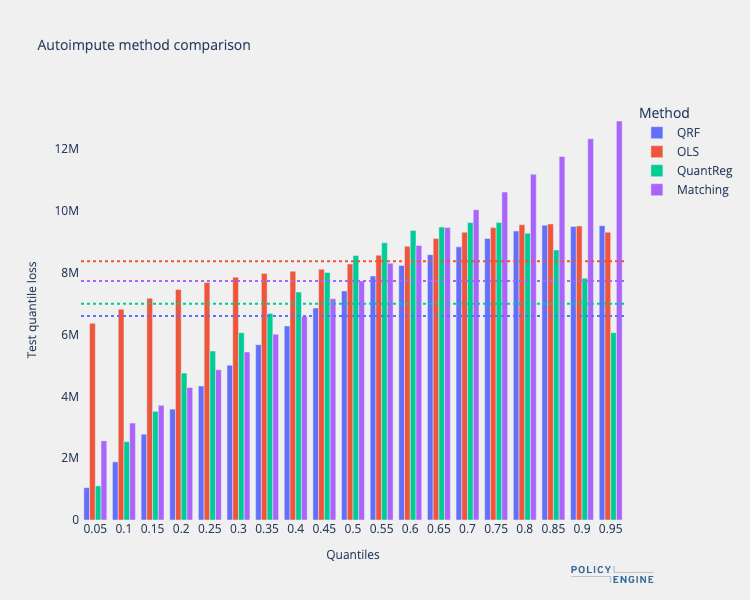
\includegraphics[width=\textwidth]{figures/quantile_loss_comparison.png}
    \caption{Cross-validation method performance at 20 equally spaced quantiles. Test quantile loss at each quantile is averaged across 5 cross-validation folds, and the dashed lines represent average quantile loss across all quantiles.}
    \label{fig:quantile_loss_comparison}
\end{figure}

We observe how QRF proves to be the best-performing model out of the four. It significantly outperforms Matching and OLS on average, while only being outperformed by QuantReg past the 80th quantile. Matching's performance presents the perfect opportunity to see the quantile loss's directional bias at work. Because Matching does not incorporate quantile information into its imputation process in any way, it will match donor and receiver units, and thus impute values identically regardless of the quantile at work. The laddering behavior observed above results from the fact that Matching's wealth imputations consistently underpredict relative to the true wealth values, and this property is increasingly favored for quantiles below the median, and increasingly penalized as quantiles approach the right end of the distribution. 

\subsubsection{Imputed wealth distribution comparisons}

\begin{figure}[h]
    \centering
    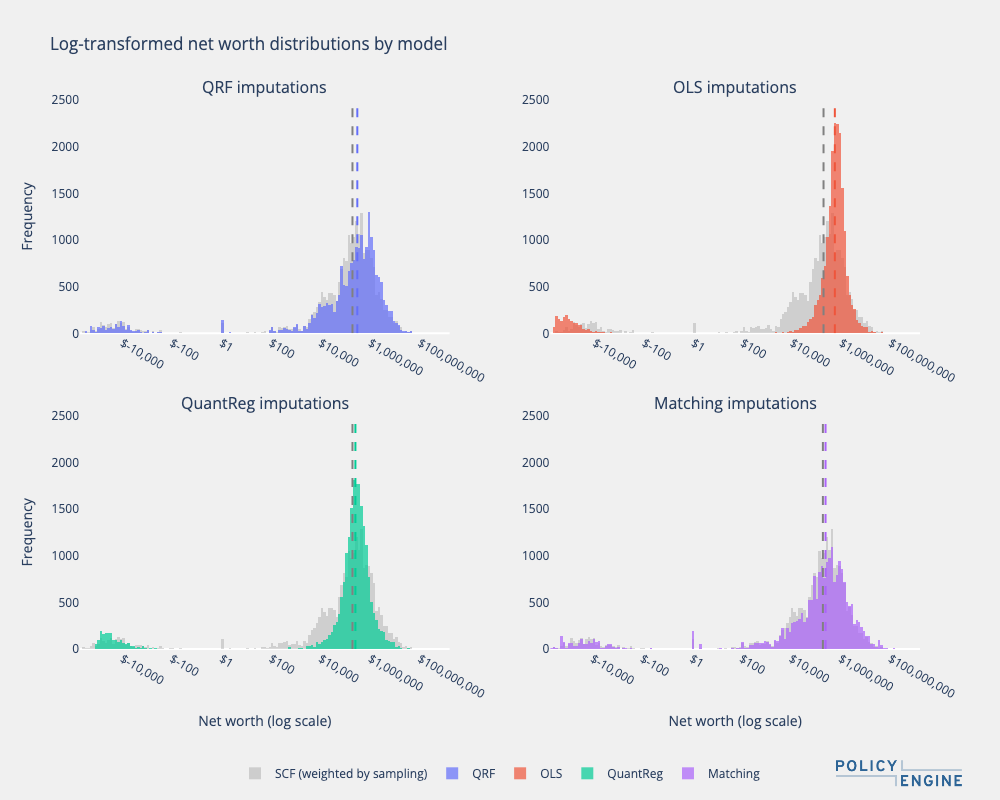
\includegraphics[width=\textwidth]{figures/imputation_distributions_method_comparison.png}
    \caption{Weight-adjusted imputed wealth distributions model comparisons, relative to the donor SCF wealth distribution. Dashed lines represent median values.}
    \label{fig:imputation_distributions_method_comparison}
\end{figure}

By visually comparing the wealth distributions resulting from imputing with each method, and comparing them to the weighted donor distribution, we gain a more comprehensive understanding of imputation performance, moving past the test quantile loss average measured on the SCF. The distribution of wealth values imputed by QRF closely resembles the original SCF distribution, suggesting that QRF is not only the best method in terms of quantile loss but also strong when achieving distributional estimates close to the true wealth distribution in the United States. Because Matching directly takes values from the donor distribution and imputes them onto the receiver, it is unsurprising that its distribution closely resembles the donor distribution. However, Matching's performance in quantile loss confirms that even if it takes the exact values from the donor, it may struggle to uncover the non-linear relationship between the different predictors and wealth values, resulting in a seemingly correct data distribution but innacurate imputation given certain household characteristics. Meanwhile, OLS and QuantReg fail to capture the variability across the distribution and impute most values at the lower or higher ends of the distribution. 

\subsubsection{Distribution of wealth by disposable income decile}

\begin{figure}[h]
    \centering
    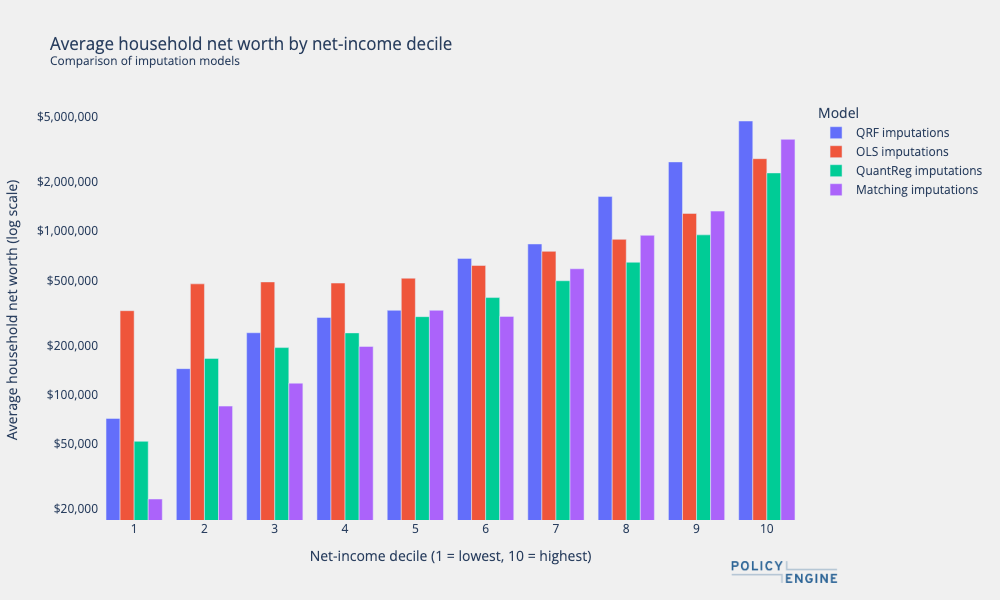
\includegraphics[width=\textwidth]{figures/imputation_comparison_by_income_decile.png}
    \caption{Average household net worth by disposable income decile model comparison. Households are divided into 10 equally sized groups based on their disposable income.}
    \label{fig:imputation_comparison_by_income_decile}
\end{figure}

These results support the observations above, with QRF presenting the most consistent and plausible relationship to disposable income, with a gradually increasing average as the deciles increase. This plot also demonstrates the caveats of the other models, for example showing the lower variability in OLS's predictions, and Matching's consistent underprediction across deciles.